\documentclass{article}

\usepackage[final]{nips_2018}

% to avoid loading the natbib package, add option nonatbib:
% \usepackage[nonatbib]{nips_2018}

\usepackage[utf8]{inputenc} % allow utf-8 input
\usepackage[T1]{fontenc}    % use 8-bit T1 fonts
\usepackage{hyperref}       % hyperlinks
\usepackage{url}            % simple URL typesetting
\usepackage{booktabs}       % professional-quality tables
\usepackage{amsfonts}       % blackboard math symbols
\usepackage{nicefrac}       % compact symbols for 1/2, etc.
\usepackage{microtype}      % microtypography

\usepackage{graphicx}
\usepackage{cite}

\title{BLACKE: Body Language Affect Classification by Keypoint Estimation}

\author{
  Undergrad-ient Descent Expedition: \\
  Jack (Xiang) Zhou, Karan Aujla, James Bie, Eric Gao, Insoo Rhee\\
  Faculty of Applied Sciences\\
  Simon Fraser University\\
  Burnaby, Canada\\
  \texttt{xza194@sfu.ca} \\
}

\begin{document}

\maketitle

\begin{abstract}
Current state of the art development in affective classification of people on visual modalities usually focuses on facial expression recognition (FER) but it has some shortcomings in its real world usage. The present work tackles the affective classification problem in body language by using keypoint estimation as a pre-processing step as opposed to previously used convolutional methods. Na\"ive neural network classifiers are trained to test for the plausibility of the approach.
\end{abstract}

\section{Introduction}

Affective Computing is a rapidly growing interdisciplinary field that is concerned with interpretations and implications of human emotion in computation. One of the most fundamental problems in Affective Computing is classification of an individual's emotional state given information about such individual on particular modalities such as text, auditory, behavioural, and visual.

For the visual modality, the present state of the art approach to addressing this problem is by Facial Expression Recognition (FER), which involves training classifiers that take images of faces as a means to identify an individual's emotional state \citep{li2018deep}, it is a successful method and current approaches can achieve near perfect accuracy ratings on testing data. However, FER is not applicable when the face of the individual is not seen or covered by objects or body limbs. 

In the present work we want to address this shortcoming by identifying the emotional state of an individual in terms of only the body language that they are exhibiting (ie. their posture). This is inherently a difficult problem for humans, in particular with respect to some emotional states over others \citep{schindler2008recognizing}. Previous work has been done on the topic using a neurologically inspired convolutional model that takes in visual data about both body language and facial expression \citep{schindler2008recognizing}.

\begin{figure}[h]
	\centering
	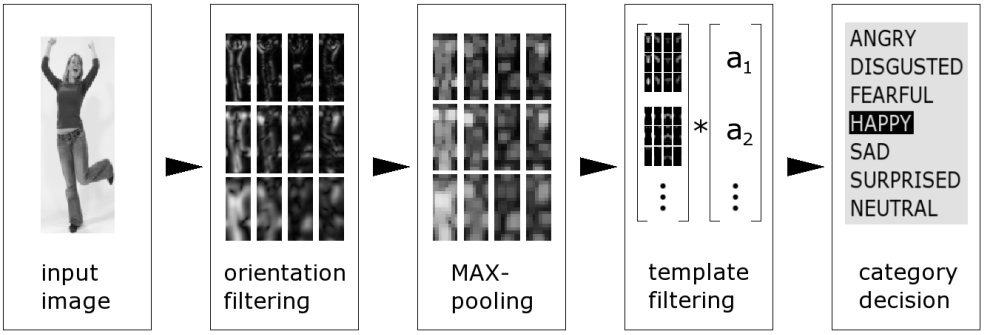
\includegraphics[scale=0.2]{schindler2008}
	\caption{Model used in Schindler et al. 2008}
\end{figure}

As seen in Figure 1, the model takes in an input image and applies orientation filtering, pooling, and template filtering on the image before feeding it into a classifier to arrive at a category decision. It is noteworthy to see that the steps taken to filter and pre-process the image are correspondent to various areas of the human visual cortex, going from low level information processing progressively to higher level information processing.

While this approach is plausible and it is able to perform just as well or better than human test subjects, the model is prone to accounting for extraneous information in the low level processing steps. The present work wishes to approach the same problem by using a different approach to pre-process the input data to a high level representation. Namely, by keypoint estimation or "skeletonization" of the body in the input image. 

The underlying motivation in play here is that when observing an image of a person, observing just the keypoints on the person preserves the relevant information regarding the person's emotional state (Figure 2).

\begin{figure}[h]
	\centering
	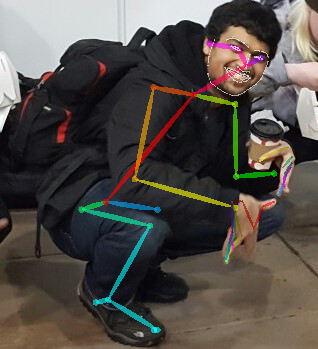
\includegraphics[scale=0.5]{kran}
	\caption{The extracted keypoints of the person's body and face contain the same amount of information regarding the person's emotional state as the full image. Image courtesy of one of our authors Karan Aujla}
\end{figure}

We hypothesize that using keypoint estimation is a feasible alternative as opposed to convolutional pre-processing to classifying emotional states based on just body language. The confirmation of this hypothesis would imply a significant dimensionality reduction to the input data for the classifier that leads more compact models and faster training times.
\newpage
\section{Approach}


\subsection{Architecture}

\begin{figure}
\centering
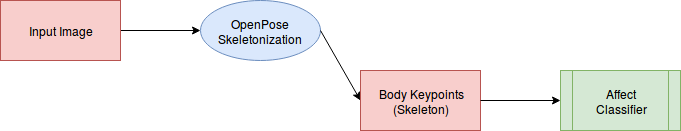
\includegraphics[scale=0.3]{kpNetwork}
\caption{The keypoints network (BLACkp)}
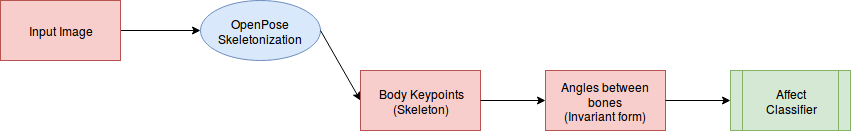
\includegraphics[scale=0.3]{angleNetwork}
\caption{The invariant form network (BLACangle)}
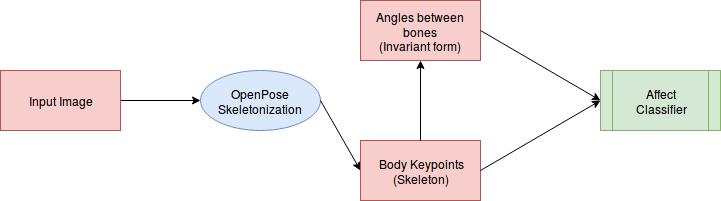
\includegraphics[scale=0.4]{mixedNetwork}
\caption{The mixed network (BLACkpangle)}
\end{figure}

We introduce the general architecture of the overall pipeline in this section. The novel and primary goal of the present work is to assign affective labels with learned patterns in body langauge. However, as we are only in the primary stage in this pursuit and we do not have a comprehensive method toward accounting for viewpoint invariance, using body posture as the primary is not very realistic. In the present work we use body language mainly as a supplement to existing facial affective labels if it is detected.

A snapshot is taken from an arbitrary visual stream and the resulting image is passed into OpenPose to detect all persons. For each person: (1) If a face was found, then it is passed into a face-based classifier for an evaluation of the affective rating vector based solely on face. (2) If a body was found, then it is passed into a body language-based classifier for an evaluation of the affective rating vector based solely on body. A weighted sum is computed between (1) and (2) for each person. If only one of (1) or (2) is found, then only that one is taken. A grand total is calculated by summing over every person's weighted sum of affective labels. The grand total will be passed into a softmax function to obtain a probability vector of the model prediction. A graphical depiction of this overall process is shown in Figure 1.

\subsubsection{Body Language Keypoint Estimation}

To extract body keypoints, we used the OpenPose system produced by the CMU Perceptual Computing Laboratory \citep{cao2017realtime} \citep{simon2017hand} \citep{wei2016cpm}

Openpose is a system the detects people in an image or video and finds the estimated location of several keypoints on their body, hands, and face. It is a capable of finding the keypoints of multiple people in the same image. Openposes’s	 basic algorithm finds each type of keypoint in all bodies at the same time and finds the connection between keypoints in a separate neural network. This program can take most image and video formats as inputs, such as jpeg, png, avi, and mp4 formats. It will output in a variety of formats depending on the flags given. For example, it can output an image with the skeletons overlaid on the people in the image, and output json files for the keypoints. In the json file, it contains the x, y coordinates of every bone detected, as well as a confidence rating for the position of each bone. Openpose can output the json in a variety of formats, such as grouping each x,y,c tuple into it’s own object. For our model, openpose is configured to output a json file containing a separate object for each bone and to normalize the coordinates to [-1,1]. Then we find the angles of each bone to ensure that the input values are position invarient

\subsection{Data}
For our dataset we contacted Beast for their dataset since they had previously created a dataset similar to what we needed for our experiment.  However, their dataset was not enough so we collected and manually labeled sample data from various online sources ranging from sports to news. We then manually labeled each sample to fit into our training model pipeline. Finally, we jittered the entire dataset to create similar but slightly varying data points. We did this by mirroring the images. We then took the dataset and ran it through a pretrained machine learning network called OpenPose which creates and approximate skeleton for the people in each of our data samples. OpenPose then returned Json file which included x and y values for each bone in the skeleton along with an associated confidence percentage. We then convert that into two distinct datasets in CSV for network processing. One of these datasets is simply a data converted and unaltered list of the bones and confidences, however the second data set is the calculated angle of each bone from it’s base. Finally the CSV files are connected together so that each row included information on all the bones that were found including position, joints and confidence levels.

\subsection{Training}
As the problem that the present model is trying to solve involve uncensored face along with body posture, it is particularly difficult to obtain relevant published datasets that are labelled and publicly available. Past research in this field involved manual construction of data from actors \citep{schindler2008recognizing}.

To address this issue, we manually construct a dataset of unlabelled images of humans with visible face and body posture by using authors of this paper as actors as well as sources on the internet. The face and body are both clearly visible in the training images. The image will not be given a label when it is fed into the training pipeline in a pseudounsupervised learning paradigm. We describe the training pipeline as follows:


The unlabelled image is first passed into OpenPose to obtain a set of posture keypoints (ie. a skeleton) of the human in the image, as well as a set of face keypoints. The face keypoints will be passed into an already trained face emotional classifier to give a ground truth affective label for the overall human in the image as informed by the face. The skeleton is then processed into an invariant form and used along with the affective label to train the body language affect classifier.

\section{Experiments}

\section{Conclusion}

\subsection{Future Work}

using a generalized linear model to deal with multiple persons instead of a simple sum

fitting LSTM to generalize into videos

accounting for Confidence in body keypoint measurements dynamically

\section{Contributions}

As with most group projects, each author of this paper contributed a considerable amount of work towards piecing together the project. Jack oversaw the project by organizing and delegating tasks for everyone as well as being the main composer of the paper and poster. Jack and James formulated the design of the overall pipeline for the models and for training the model. Karan worked with existing models for body posture keypoint extraction and implemented the top level program. Eric and James are the main contributors to data collection and piecing together a custom dataset for the project. Insoo and Jack worked on designing and implementing the model for mapping body keypoints to affective labels.

We would also like to thank Professor Angelica Lim for consultations and guidance toward the design and theoretical groundwork for the project.

\bibliography{references.bib}
\bibliographystyle{plain}

\end{document}
